\documentclass[12pt]{report}

\usepackage[hidelinks]{hyperref}
\usepackage{graphicx}
\usepackage{cite}
\usepackage[toc,page]{appendix}







\title{Classroom Management Handbook}
\author{Lyron Winderbaum}

\begin{document}

\maketitle

\tableofcontents

\chapter{Introduction}

This document is written as a reference manual of strategies for classroom behaviour management. The goal is that a teacher could consult this document in order to prompt them on strategies they might have forgotten about or not thought of. The language used will be deliberately concise, and is not intended to be comprehensive --- quite the opposite, it is intended as a memory prompt, not an encyclopedia.

This handbook is organised by chapters. Chapters \ref{chap:preventative}, \ref{chap:supportive} and \ref{chap:corrective} introduce a list of strategies, each as a section or sub-section.
Again this list is not intended to be comprehensive, but rather represents a selection of strategies that resonate with me personally. These chapters seperate strategies into the three broad categories of \cite{Charles2002}: preventive, supportive, and corrective, respectively. In the interests of brevity I will keep the descriptions of these strategies minimal, only providing examples and further elaboration in later chapters and appendices. Chapter \ref{chap:video_examples} discusses some of the videos shown in lectures in the context of these strategies, providing some examples of their use in practice. Finally, Chapter \ref{chap:theories} discusses some popular theorists, and how the theory relates to the strategies.

\textbf{Disclaimer 1:} I've written this document from my perspective, so any statements that are not explicitly referenced to be otherwise are my personal opinion and nothing more.

\textbf{Disclaimer 2:} In some places I might use language such as "It is wrong to...", "You should...", etc. --- it is important to recognise that every situation comes with it's own intricacies and context and that no such absolute statements can ever be universal.










\chapter{Preventative Strategies}
\label{chap:preventative}

These are strategies that apply when there is no specific misbehaviour being addressed, but rather are preventative in the sense that they describe approaches that can help prevent problematic misbehaviour ever occurring in the first place. These are by far the most preferable strategies to be using and so should always be the place to start. Other strategies should only be attempted if the preventative strategies have already failed. 

\section{Praise}
\label{sec:praise_p}

Praise your students! Some students may never have been praised before, don't underestimate the power it can have. Be specific with your praise --- refer to something specific they have done, whether it be some work or their self-regulation, whatever. Most importantly: \textbf{be genuine}. Warning: if your praise is not genuine, your students will know, and they will not appreciate it.



\section{Don't Assume}
\label{sec:dont_assume_p}

You don't know what your students have gone through at home or in their lives. You don't know if their misbehaviour is malicious or is just coming from learnt emotional reactions they have no control over. \textbf{You don't know} --- don't assume. When confronted by misbehaviour, don't immediately react with criticism or condemnation --- instead, train your initial reflex reaction to be one of compassionate calm. Warning: If you make assumptions about a students misbehaviour, they will pick up on it and they will not appreciate it. Conversely, if you keep an open mind and focus on reacting compassionately, you could open the door to building rappor (\ref{sec:rapport_p}). This can also help in feeling genuine when giving praise (\ref{sec:praise_p}) and sympathy.

This strategy is obviously easier said than done, but it is an important one to keep in the back of your mind as you work on your personal development.



\section{Show Interest}
\label{sec:show_interest_p}

Be interested in what is going on in your students lives. This is a natural extension of not assuming and being compassionate (\ref{sec:dont_assume_p}), but can also lead to learning about what is important to your students and this can allow you to design relevant (\ref{sec:relevance_p}) and interesting (\ref{sec:fun_p}) lessons for them.



\section{Use Names}
\label{sec:use_names_p}

Learn the students names. Use them. Students will appreciate the effort you have gone too and the care for them you have demonstrated by doing so (\ref{sec:show_interest_p}). Similarly to praise (\ref{sec:praise_p}), the impact of this strategy is not to be underestimated.



\section{Rapport with Students}
\label{sec:rapport_p}

Praise (\ref{sec:praise_p}), using names (\ref{sec:use_names_p}) are both ways of showing interest (\ref{sec:show_interest_p}) in your students. When you do these things you can develop a rapport with the students that is a powerful, and valuable thing.



\section{Establish Routines and Procedures}
\label{sec:routines_p}

Habit is powerful. If you can instill routines into you class early, you can save yourself alot of headache in the future.

\subsection{Democratic setting of classroom practices}
\label{sec:democratic_setting_of_routines_p}

Discuss classroom practices with students --- give them an opportunity to share their opinions. If they buy into the rules and routines by having influence on deciding what they are, they will have a sense of ownership, and be more likely to follow those rules and routines.



\section{Use of Language}
\label{sec:language_p}

The words we choose and the way we speak can have a profound impact on how people perceive us, and students can be particularly sensitive to this.

\begin{itemize}
  \item Use inclusive language --- don't assume (\ref{sec:dont_assume_p})!
  \item Use clear and concise sentences.
  \item Use appropriate vocabulary.
  \item Articulate well, and at an appropriate volume.
  \item If you have any English as an additional language students, or students with hearing impairments, ensure they have access to the information: 
  \begin{itemize}
    \item Use sign language (if possible), 
    \item Provide translations (if possible), 
    \item Speak slowly and clearly, 
    \item Articulate deliberately,
    \item Do the above without being condescending.
  \end{itemize}
\end{itemize}

\subsection{Clear Instructions}
\label{sec:clear_instructions_p}

It is particularly crucial to be clear when delivering instructions. For verbal instructions,
\begin{itemize}
  \item Be heard: Ensure there is silence before delivering instructions (same as \ref{sec:start_well_p}).
  \item Ensure students have access to all the information they need: If you are asking them to interpret an image, ensure they can see the image, etc. 
  \item Use clear verbs so it is clear what they are expected to do: "Draw", "Calculate", "Write", etc.
\end{itemize}

\subsection{Clear Materials}
\label{sec:clear_materials_p}

Delivering instructions clearly equally applies to written instructions, not only verbal instructions (\ref{sec:clear_instructions_p}). Appropriate (easy to read) fonts and vocabulary should be used for handouts, etc.



\section{Non-verbals}
\label{sec:non_verbals_p}

Similar to the use of language (\ref{sec:language_p}), non-verbals such as body language, positioning, attitude, facial expressions, etc. have a big impact on how you are perceived. 

\subsection{Enthusiasm}
\label{sec:enthusiasm_p}

The students can tell if you are genuinely enthusiastic about the lesson, about the topic, about seeing them, and enthusiasm is infectious.



\section{Preparation}
\label{sec:preparation_p}

This is an important strategy. If you put in work preparing for your classes, it will pay off both because the preparation itself, but also because your students will recognise the work you have put in for them, and appreciate it. 

\subsection{Relevance}
\label{sec:relevance_p}

Make material (lessons, activities, etc.) that is relevant to your students lives. If you have some rapport (\ref{sec:rapport_p}) with your students you can ask them what they are interested in and design lessons and activities around their interests.

\subsection{Fun}
\label{sec:fun_p}

Design interesting and fun lessons and activities! Similar to relevance (\ref{sec:relevance_p}) if you have some rapport (\ref{sec:rapport_p}) with your students you could try asking them what they think might be fun and try designing a lesson around that.

\subsection{Structure}
\label{sec:structure_p}

Design structured lessons. This is vague and broad, as it can be done in many ways, but having prepared an appropriate amount of activities and a structure linking them together in a lesson cannot be overstated in it's usefulness.



\section{Start Well}
\label{sec:start_well_p}

Before beginning a class, ensure that you have the classes' full attention, and complete silence. This is an important routine (\ref{sec:routines_p}) to set, in that if you can get your class into the routine of falling silent at the beginning of a class, it will make starting well much easier for you.

\subsection{Starter Activity}
\label{sec:starter_acivity_p}

A starter is a structured (\ref{sec:structure_p}) way to start a lesson, often it is a short (5-10min) activity that is fun, engaging, and easy, and serves the function of transitioning (\ref{sec:managing_transitions_p}) the students from being out of class or a in a different class to being in class, and in the appropriate mindset.




\section{Flow/ Momentum}
\label{sec:flow_p}

Once you have started well (\ref{sec:start_well_p}) and gotten the students engaged (see \ref{sec:relevance_p}, \ref{sec:fun_p}) you have gotten the momentum of the class started, then you need to maintain this "flow". This can be done by use of structure (\ref{sec:structure_p}) and managing transitions well (\ref{sec:managing_transitions_p}), but the exact process for doing this is difficult pin down because it is so context dependant. It involve a quality some refer to as "withitness" (\ref{sec:kounin_theory}), which more or less is an awareness of the situation and the ability to see problems coming up before they occur and managing them before they derail the class --- this takes practice, and similar to "don't assume" (\ref{sec:dont_assume_p}) is something to monitor and keep in the back of your mind as you work on your personal development as a teacher.

\subsection{Managing Transitions}
\label{sec:managing_transitions_p}

Starting well (\ref{sec:start_well_p}) is a key example of a transition: from out-of-class to in-class. But there will be transitions inside the class as well from one activity to another, and these are the key points where momentum can easily be lost. To maintain good behaviour in your class being prepared for these transitions is crucial. Similar to starting well (\ref{sec:start_well_p}) and delivering clear instructions (\ref{sec:clear_instructions_p}) a good strategy for managing transitions is to ensure quiet and complete attention before beginning the next activity, and insisting that this becomes routine (\ref{sec:routines_p}). 



\section{Mix different activities}
\label{sec:mix_differnt_activities_p}

If you do the same kind of activity over and over, it will get boring. Mix it up! Use a variety of approaches and activities (\ref{sec:blooms_taxonomy}, \ref{sec:gardner_theory}).



\section{Manage your Time}
\label{sec:manage_your_time_p}

Time management is important. Reflect on how you have been spending your time in class, and if neccessary make adjustments. 



\section{Model appropriate behaviors}
\label{sec:model_behaviours_p}

Don't be a hypocrite. Simple, if you are going to ask the students to behave a certain way --- adhere to the same standard yourself.


























\chapter{Supportive Strategies}
\label{chap:supportive}

These are for situations when the misbehavior is not so severe as to require being addressed directly. Instead, the students can be encouraged and guided via supportive strategies to adopt more productive and helpful behaviours. This is preferable to addressing misbehaviour directly (correctives), and should be attempted first with correctives only being resorted too if the supportive strategies have already been exhausted.


\section{Praise}
\label{sec:praise_s}

Although praise can be preventative (\ref{sec:praise_p}), it can also be used as a supportive strategy. If you have students who sometimes meander off task, praising their on-task behaviour can encourage more on-task behaviours.  

\subsection{Peer Praise}
\label{sec:peer_praise_s}

One of the strongest forms of praise you can offer a student is that of their peers --- if a student has done something particularly well, encourage their peers to applaude, or similar.
Warning: certain types of students may react badly to this, use with discretion.

\subsection{Acknowledge others good behaviour}
\label{sec:acknowledge_good_behaviour_s}

In the case of attention seeking students whose misbehaviour is motivated by wanting your attention, praising and giving your attention to other students who are on-task can encourage the attention seeking students to mimic on-task behaviours as they can see others getting attention for those behaviours.

VIDEO REFERENCE.



\section{Use Names}
\label{sec:use_names_s}

Using names can be preventative (\ref{sec:use_names_p}), but it can also be used as a supportive strategy. By using names when giving praise (\ref{sec:praise_s}) for example, you can reinforce that you are noticing a specific students on-task behaviour, strengthening that reinforcement by showing that you know their name and care enough to have remembered it.



\section{Scaffolding}
\label{sec:scaffolding_s}

If students are losing interest and going off-task as a result of trying, but struggling to complete, a task offer help in completing the task. If you can give them a sense of success by helping them complete the task, keeping them in the ZPD (\ref{sec:zpd_theory}). Often this will result in a feeling of accomplishment on their part, and will encourage on-task behaviour.



\section{Proximity ("The Whisper Technique")}
\label{sec:proximity_s}

Proximity can be used as a supportive strategy by using it to deliver help (\ref{sec:scaffolding_s}) privately. Often if you offer help publically (in front of the students classmates) it can be embarressing for them and they might not be receptive. In contrast, using proximity to deliver aid in a whisper that is not as public can improve the chances that the student will be receptive to the scaffolding (\ref{sec:scaffolding_s}).



\section{Eye Contact}
\label{sec:eye_contact_s}



\section{Tactical Ignoring}
\label{sec:tactical_ignoring_s}

This is the other half of the coin to the acknowledging good behaviour (\ref{sec:acknowledge_good_behaviour_s}) strategy for dealing with attention seeking students. You can deliberately ignore off-task behaviour, giving your attention instead to on-task behaviour and the misbehaving students may begin to feel left out, and start to cooperate in an attempt to be included.

VIDEO REFERENCE: Attention seeking students. 



\section{Wait time.}
\label{sec:wait_time_s}

Broken Sentencees --- pause to get attention (VIDEO: Manage that lesson (chemistry year 8)

"Canter's "Broken Record"" in Figure~\ref{fig:correctiveHierarchy}, 


\section{Challenge Students}
\label{sec:challenge_s}

Certain misbehaviours can be turned around by challenging the student to do what they say, etc. 

VIDEO: French Teacher? I challenge you! 

\section{Use humour to depotentiate}
\label{sec:humour_s}

Is a students misbehaviour has led to confrontation or tension in the classroom, humour can sometimes be used to depotentiate the situation.

























\chapter{Corrective Strategies}
\label{chap:corrective}

There will come times when students misbehave to a point that their misbehaviour must be addressed directly and can no longer be managed by supportive strategies alone --- this is were corrective strategies apply. Even so, such measures should always be applied with every possible attempt to avoid escalation. The harsher the corrective used, the more likely it is to result in escalation, and so it is always preferable to use the softest corrective possible that manages the behaviour. See Figure~\ref{fig:correctiveHierarchy}. I will (roughly) organise the strategies in this chapter in increasing order of "harshness".

It is also important to note the special case of chronic misbehaviour --- in this case it is particularly important to try to understand the underlying cause of the misbehaviour. There are a number of approaches to this, one of which is Dreikurs' social discipline model (\ref{sec:dreikur_theory}).


\begin{figure}[p]
\begin{center}
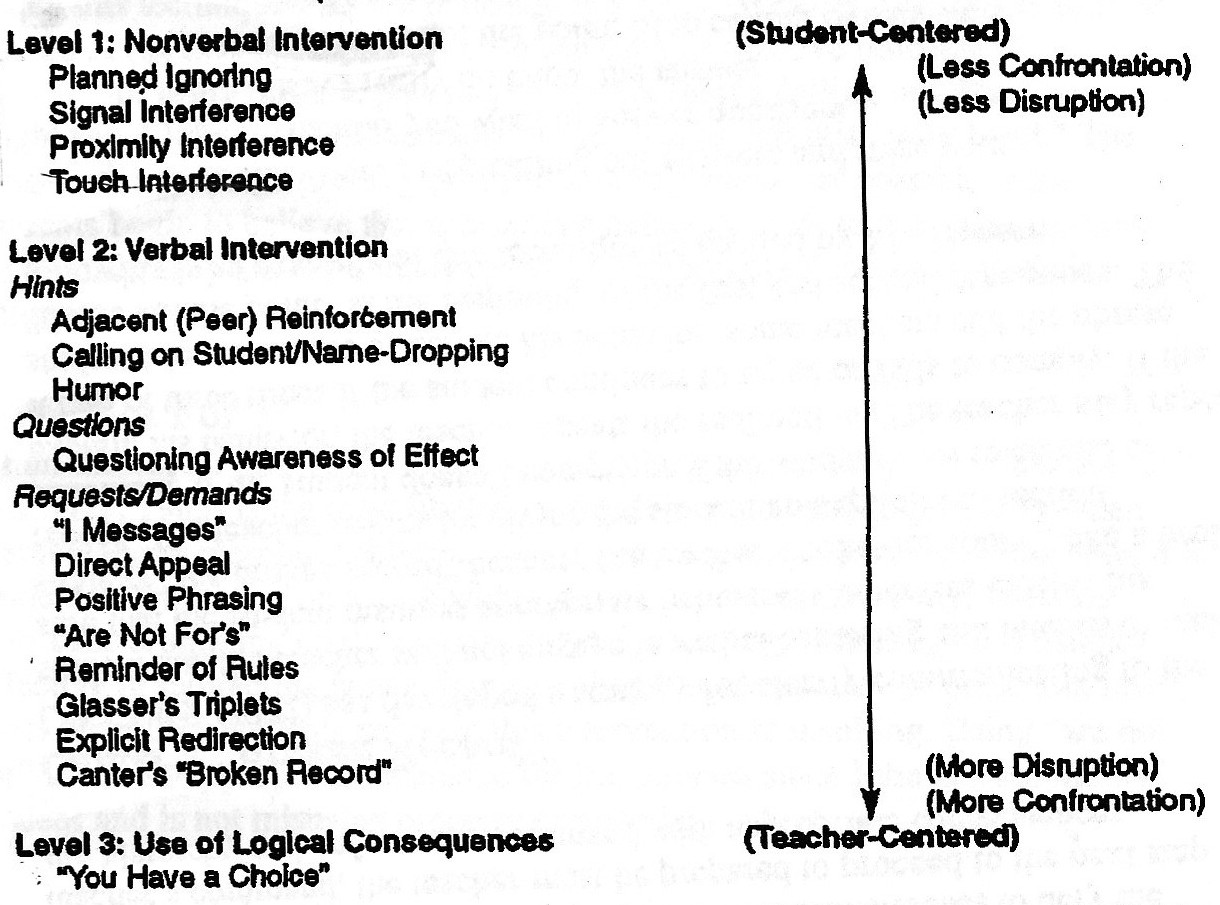
\includegraphics{./images/correctiveHierarchy.jpg}
\end{center}
\caption{Hierarchy of Management Intervention Diagram \cite{Levin2005} showing a list of corrective strategies, ranked in increasing order of harshness. Some of these are not applicable (such as touch), and others have already been covered as supportive strategies (there is a grey area betwene supportive and soft corrective strategies) such as "Planned Ignoring" (\ref{sec:tactical_ignoring_s}), "(Peer) Reinforcement" (\ref{sec:peer_praise_s}), and "Humour" (\ref{sec:humour_s}), but many others on this list will be discussed in this chapter. The general strategy of applying correctives to a misbehaviour would be to work your way down this list until you find a strategy that manages the misbehaviour and then stop. The goal is to avoid overshooting and using an unneccessarily harsh corrective in any given case. \label{fig:correctiveHierarchy}}
\end{figure}


\section{Eye Contact}
\label{sec:eye_contact_c}

This can be a nice soft corrective, just catch the misbehaving students' eye from accross the room and hold their gaze for a moment in order to communicate that you have noticed their behaviour\footnotemark. 



\section{Proximity ("The Whisper Technique")}
\label{sec:proximity_c}

Although typically proximity would be used supportively (\ref{sec:proximity_s}), it can also be used as a corrective by simply placing yourself (the teacher, a figure of authority) close to the misbehaviour\footnotemark[\value{footnote}].

Although included as a soft corrective in Figure~\ref{fig:correctiveHierarchy} ("Proximity Interference"), be warned: if combined with a direct appeal (\ref{sec:direct_appeal_c}) or other corrective in the wrong situation or with the wrong student, this could quickly lead to escalation and confrontation. Even when used on it's own proximity can be very intimidating and could provoke a strong reaction from certain students, use caution and gauge the situation before applying this strategy.



\section{Use Names}
\label{sec:use_names_c}

"Calling on Student/Name-Dropping" in Figure~\ref{fig:correctiveHierarchy}, 

\footnotemark[\value{footnote}]

\section{Questioning}
\label{sec:questioning_c}

"Questioning Awareness of Effect" in Figure~\ref{fig:correctiveHierarchy}, 



\section{Gordons I-Messages}
\label{sec:i_messages_c}

Thomas Gordon (\ref{sec:gordon_theory}) suggested a three step process for initiating a conversation with a student in a non-confrontational way (at least that is the intention!)  about behaviour the teacher is unhappy with:
\begin{itemize}
  \item Describe the disruptive behaviour.
  \item Describe the effect on the teacher and/ or other students.
  \item Describe your feelings about the behaviour.
\end{itemize}


\section{Direct Appeal}

\section{Reminder of Rules}

\section{Glassers Triplets}



\section{Arrange to talk privately with student about their misbehaviour}
\label{sec:private_talk_c}

\section{Give choice}
\label{sec:give choice_c}

\section{Apply Sanctions}
\label{sec:sanctions_c}



\footnotetext{As with most soft correctives, the best use would be seamlessly interwoven into your delivery without impacting on the flow of the lesson (\ref{sec:flow_p}, \ref{sec:kounin_theory}.}













\chapter{Video Examples}
\label{chap:video_examples}

Preparation (VIDEO: Praise and Preparation, Amy)

 Amy is a good example of structure this (VIDEO REFERENCE).

Non-verbals such as being happy to see the students (VIDEO: Talk too much).
A fantastic example of non-verbals this is simply being (genuinely) happy to see the students.
(VIDEO REFERENCE). Warning: Similar to with praise (\ref{sec:praise_p}), being genuine is crucial in this example --- if you are not genuine the students will be able to tell.



\chapter{Theories and Theorists}
\label{chap:theories}


\section{Blooms Taxonomy}
\label{sec:blooms_taxonomy}

% \begin{figure}[h]
% \begin{center}
% \includegraphics{./images/circle.gif}
% \end{center}
% \caption{Blooms Revised Taxonomy Wheel \label{fig:bloomsTaxonomy}}
% \end{figure}



\section{Garder's Multiple Intelligences}
\label{sec:gardner_theory}



\section{Thomas Gordon}
\label{sec:gordon_theory}

The approach of Thomas Gordon is centred on "the importance of developing meaningful mutually beneficial relationships" (\href{https://en.wikibooks.org/wiki/Classroom_Management_Theorists_and_Theories/Thomas_Gordon}{wiki page}). Gordon claims that in relationships each participant (in this case students and teachers) bring their own values and needs and these will disagree and result in conflict. Gordon suggests that to resolve such conflicts the first step is to identify who "owns" the problem --- that is, which is the disgruntled party. Then:
\begin{itemize}
  \item If the student "owns" the problem, the teacher should engage in "active listening" --- that is they should listen to the students grevance and genuinely try to understand and empathise with their frustrations (\ref{sec:show_interest_p}, \ref{sec:dont_assume_p}, \ref{sec:non_verbals_p}).
  \item If the teacher "owns" the problem, then they should use an "I-message" (\ref{sec:i_messages_c}) to initiate a conversation in a non-confrontational way.
\end{itemize}
Finally, the object in Gordons framework is to acheive a solution in which both parties have contributed and feel invested in, similar in principle to the buy-in discussed in \ref{sec:democratic_setting_of_routines_p}.


\section{Vygotsky's Zone of Proximal Development (ZPD)}
\label{sec:zpd_theory}


Amongst other things, Vygotsky proposed the ZPD model for learning. The ZPD model claims that all learning occurs in the ZPD, which is defined as the set of tasks and activities or concepts that the students cannot complete or understand without help, but with help can. This is the essence of the concept behind scaffolding (\ref{sec:scaffolding}). If students are given tasks so difficult they cannot complete them successfully even with help from the teacher, or they are given tasks so easy they can complete them easily on their own, they will not learn anything, and they will likely quickly lose interest in the lesson, become bored, and misbehave. Only if they are given tasks of just the right level of difficulty, and are given assistance in completing those tasks, will they learn and engage.



\section{Jacob Kounin}
\label{sec:kounin_theory}

Jacob Kounin wrote alot about the effect a teacher can have on misbehaviour in their class through mostly preparatory techniques (\ref{sec:preparation_p}) such as structuring lessons well (\ref{sec:structure_p}), with a focus on what he refered to as "Lesson Movement" (\ref{sec:flow_p}) and managing transitions (\ref{sec:managing_transitions_p}). Kounin is the one who coined the term "withitness".

Also noticed the "Ripple Effect", and sugggested a broad categorisation of attributes a teacher should focus on developing in their lessons: Withitness, Overlapping, Momentum, Smoothness and Group Alerting. For more detail refer to \href{http://universityofhullscitts.org.uk/scitts/site/pt/behaviour/kounin.html}{this website}.

\section{Dreikurs' Social Discipline Model (in the context of chronic misbehaviour management)}
\label{sec:dreikur_theory}

Very breifly, Dreikurs' Social Discipline Model can be used to diagnose and approach chronic misbehaviour by first identifying the goal of the behaviour, which is usually one of:
\begin{itemize}
  \item Attrating Attention,
  \item Power,
  \item Revenge, or
  \item Escape by Withdrawl.
\end{itemize}
What the goal of the behaviour is can often be diagnosed by observing the effect the behaviour has on the teacher. If the teacher feels:
\begin{itemize}
  \item Minor annoyance and frustration, then the goal was likely attention seeking.
  \item Personally challenged, then the goal was likely power. 
  \item Deeply hurt, then the goal was likely revenge.
  \item Like giving up, then the goal was likely escape by withdrawl.
\end{itemize}
The most common goals of chronic misbehaviour are attracting attention, and escape by withdrawl, and there are two broad approaches to addressing chronic misbehaviour which can be roughly matched against these two goals:
\begin{itemize}
  \item Relationship Building (to address mostly attention seeking behaviours): through building rapport (\ref{sec:rapport_p}) and having private conversations (\ref{sec:private_talk_c}) with the student, often acceptable behaviours can be negatioated where both the teachers and the students needs are being met.
  \item Breaking the cycle of discouragement (to address mostly escape by withdrawl behaviours): through scaffolding (\ref{sec:scaffolding}), careful design of lessons and praise (\ref{praise_s}), the student can be given a feeling of success which can sometimes break through their cycle of discouragement.
\end{itemize}
  








\begin{appendices}

\chapter{Elaboration on Stategies with Examples}

\section{Manage your Time}
Examplees of time-management --- have you been spending all your time speaking to the same students, are there some that have not had a chance to speak to you or get your attention? Have you been spending alot of time in class doing things that could be done beforehand (\ref{sec:preparation_p}), like writing on the whiteboard for example? Are these important? If the answer to any of these leading questions is yes, considering managing your time differently --- explain that you will only spend a certain amount of time with each student s


\chapter{More Theories and Theorists}


\section{Maslow's Hierarchy of Needs}


\section{Glasser's Choice Theory}


\section{Piaget's Developmental Stages}



\section{Skinners' Operant Conditioning}

\section{Cognititive Load Theory}

Cognitive Load Theory, originally attributed to (Sweller?), is a learning model in which it is hypothesises that the number of new or unfamiliar concepts that can be held in working memory at any given time is limited. The practical consequences of this are similar to those of ZPD, in that the amount of work, the number of new concepts, provided to students need to be metered out at an appropriate rate. If too much information is provided all at once, the students will go into cognitive (over-)load, and will simply zone out --- and likely misbehave.


\end{appendices}

\bibliography{references}{}
\bibliographystyle{apalike}


\end{document}